\subsection{Expressivity of ANIMO models}\label{sec:animo-drosophila}
While allowing for a low degree of freedom in setting the parameters of models,
ANIMO is still precise enough to describe the behavior of complex networks.
The results obtained with ANIMO are comparable to the ones obtainable with other modeling
approaches, but the modeling process in ANIMO requires considerably less expertise about the formal foundations.
To demonstrate this, Figure~\ref{subfig:drosophila-model}
represents an ANIMO model of the drosophila circadian clock based on the work by~\cite{drosophila-ode-model}, where ordinary
differential equations (ODEs) were used.
The cyclic behavior of the circadian clock is based on the alternating formation and destruction of the CYC/CLK (cycle/clock) protein complex.
This is in turn regulated by a series of proteins which are produced as a consequence of CYC/CLK formation. The CWO (clockwork orange) protein
is central to the network working, as it degrades the mRNA for most of the involved proteins, thus acting as an inhibitor counterbalancing
the action of CYC/CLK.
The positive influence of the light-regulated cryptochrome CRY on the degradation of TIM is a consequence of the passage between light and dark, allowing
the circadian clock to synchronize to a time zone (see Suppl. Sect.~\ref{suppl:repressilator}).


\def\drosophilaGraphScale{0.069}%0.123}

\begin{figure}[!htpb]
\begin{center}
\subfloat[\label{subfig:drosophila-model}]{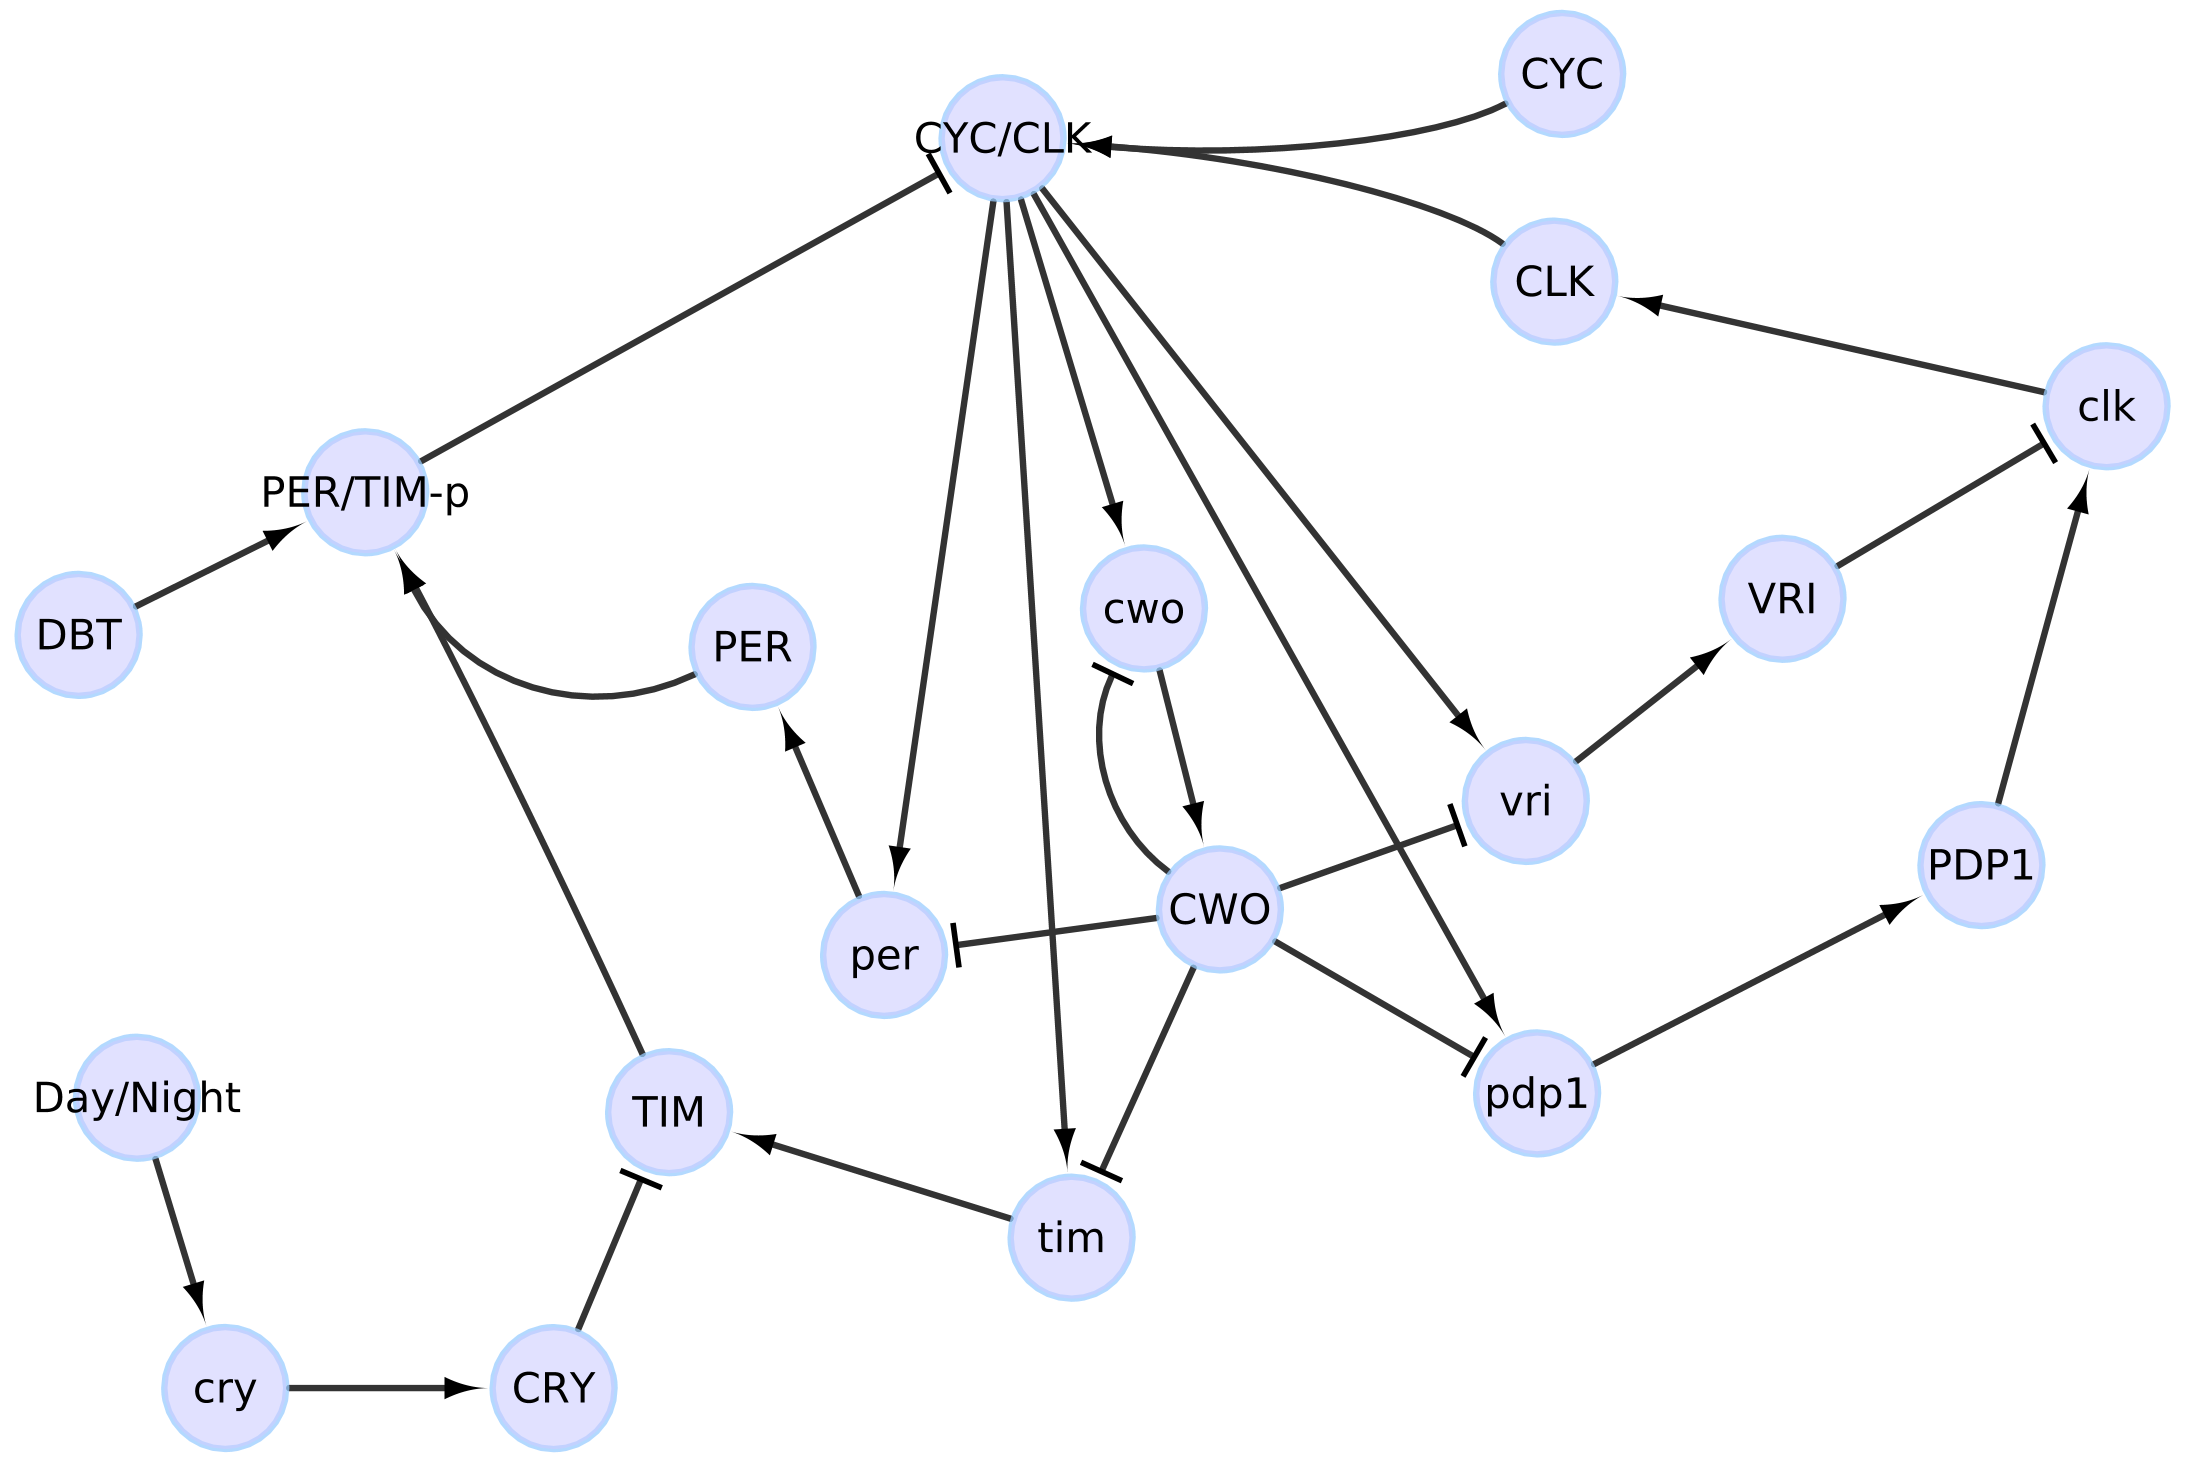
\includegraphics[width=0.49\textwidth]{images/drosophila_model5}}\ %0.85\textwidth
\subfloat[\label{subfig:drosophila-mrna}]{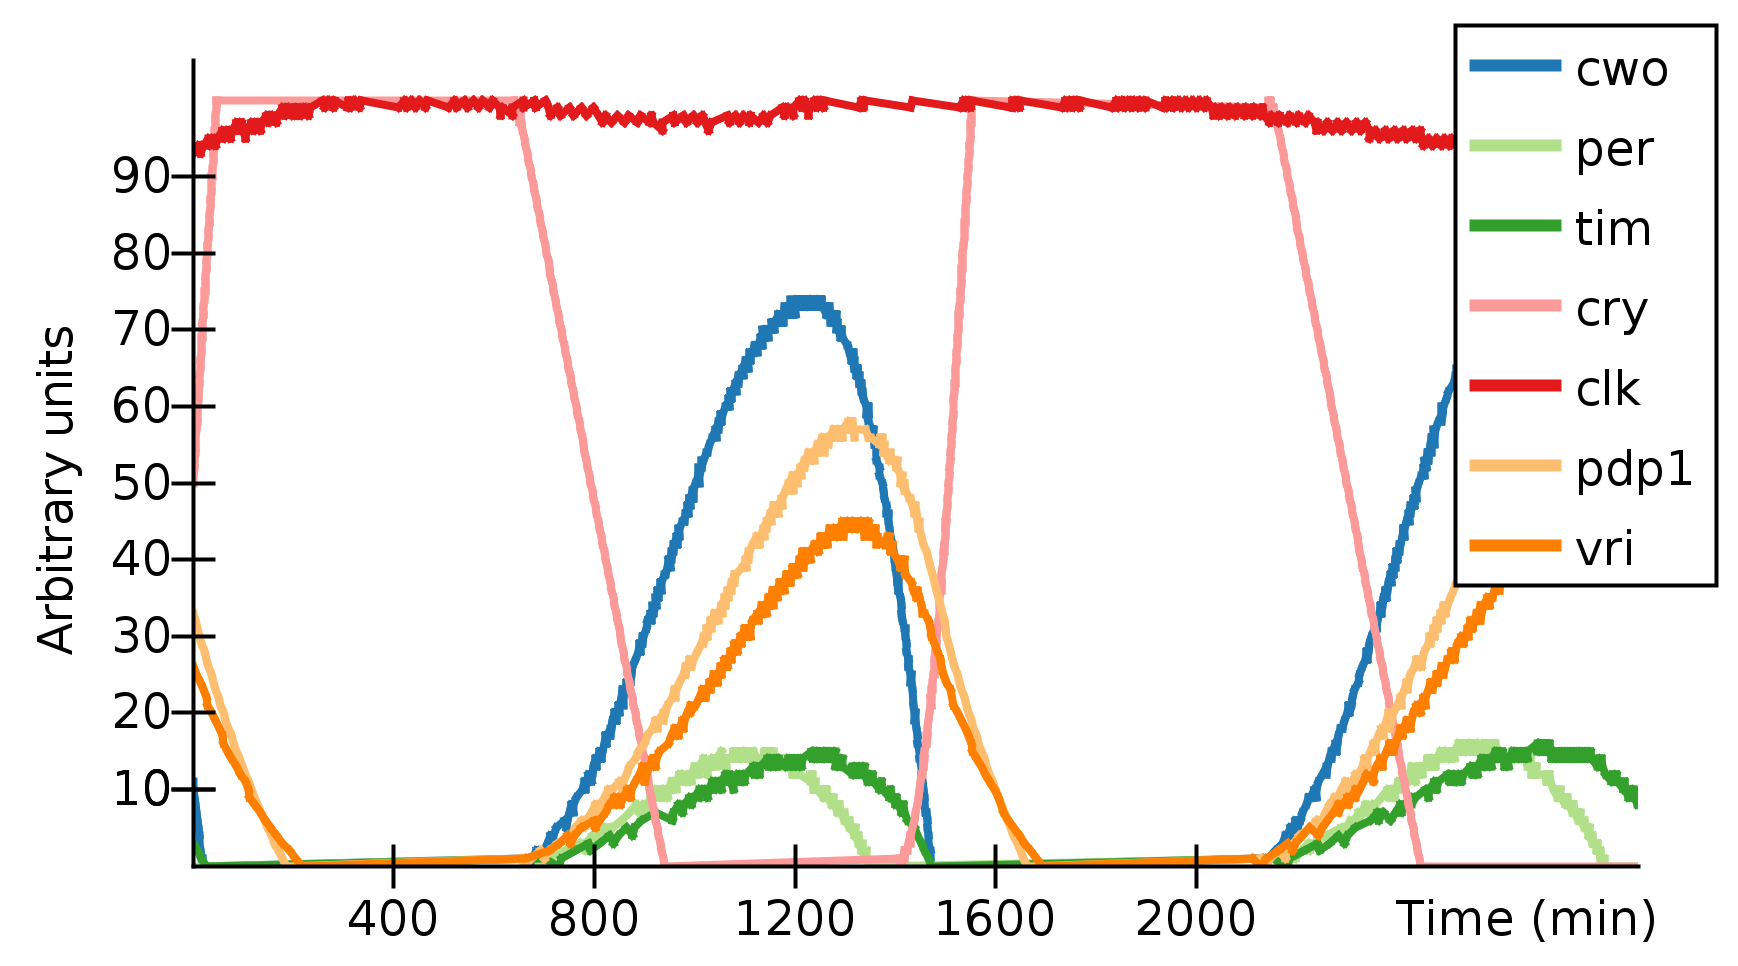
\includegraphics[scale=\drosophilaGraphScale]{images/drosophila_graph2}}\ 
\subfloat[\label{subfig:drosophila-proteins}]{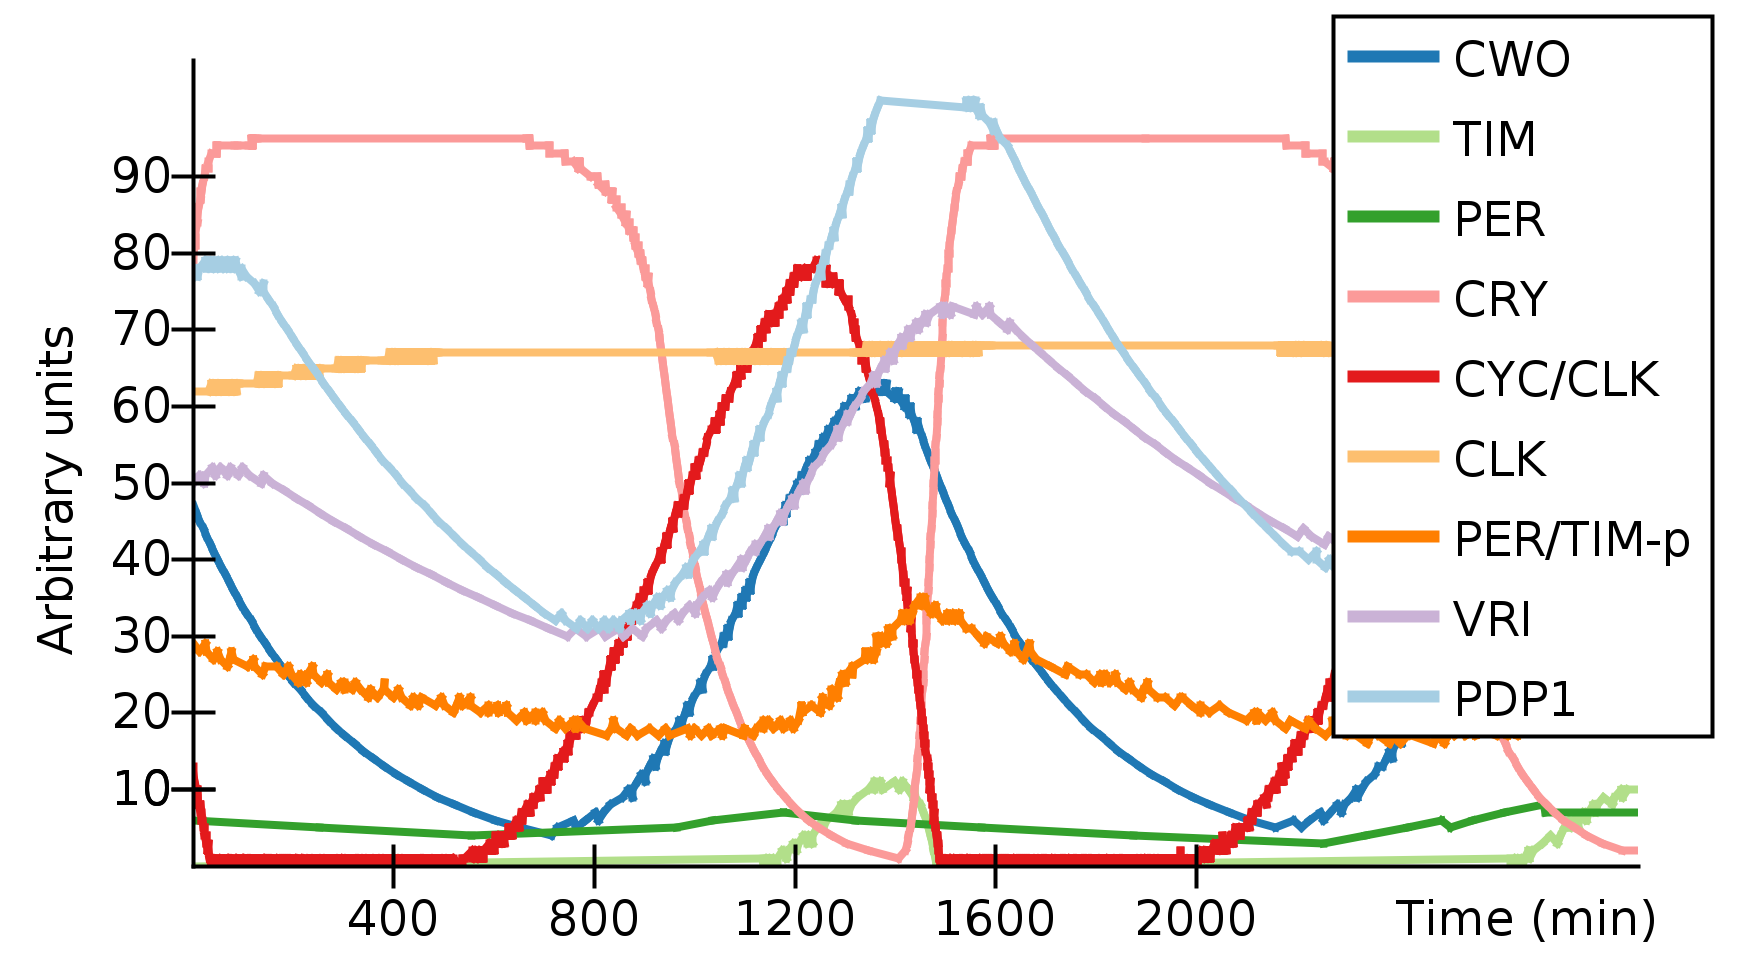
\includegraphics[scale=\drosophilaGraphScale]{images/drosophila_graph1}}
\end{center}
\caption{ANIMO model of the drosophila circadian clock {\bfseries \protect\subref{subfig:drosophila-model}}.
Negative auto-loops on the nodes of the circadian clock network
are also present in the model, following the example of the model by~\cite{drosophila-ode-model}, but are not
represented here only for cosmetic purposes. Naming conventions follow the same rule
as in the original model, with lower-case names representing mRNA, and upper-case names indicating proteins.\\
ANIMO plots of the concentration of
mRNA~{\bfseries \protect\subref{subfig:drosophila-mrna}}
and proteins~{\bfseries \protect\subref{subfig:drosophila-proteins}} over a period of 48~hours.
Oscillations are shown here on an absolute scale, while the graphs in~\citep{drosophila-ode-model}
are based on relative scales, where each series was normalized considering
local minimum and maximum values.}\label{fig:drosophila}
\end{figure}


We see in Figures~\ref{subfig:drosophila-mrna} and~\ref{subfig:drosophila-proteins} that the modeling
power of ANIMO is sufficient to reproduce the cyclic behavior of the model.
In particular, the oscillations exhibited by the two models show the same periods and phases.
Moreover, the ANIMO user interface allows for intuitive \emph{in silico} knock-out experiments,
by manually disabling a node in the model. Such experiments have been done before~\citep{drosophila-ode-model} and
give similar results in our model.
% The model we present here is to be intended only as an example of how a rapidly sketched ANIMO model can help
% in reasoning over existing network models, and not as a complete explanation of the circadian clock network.
% Producing a model that closely fits all experimental conditions for the studied network would be outside the scope of this paper.



\subsection{Case study: using ANIMO to generate hypotheses}\label{subsec:case-study-larger}
In order to validate our modeling approach,
we construct a larger model of the signaling network downstream of TNF$\alpha$ and EGF, and formalize crosstalk between the pathways.
 We first modeled the two pathways in isolation~(Figs.~\ref{fig:large-model-tnf}, \ref{fig:large-model-egf}),
using information on protein interactions from
the KEGG~\citep{kegg} and phosphosite~\citep{phosphosite} databases. These models were fitted to the data
from the works by~\citet{pathway-compendium,pathway-autocrine}.
We then merged the two pathways into a single model and added autocrine crosstalk between the pathways that has been
reported previously~\citep{pathway-autocrine}.
Briefly, stimulation with TNF$\alpha$ leads to a rapid release of TGF$\alpha$ ({\sf TGFa} in the model), which activates the EGF receptor ({\sf EGFR}).
This activation causes secretion of IL-1$\alpha$ ({\sf IL-1a}) at later time points.
The effect of IL-1$\alpha$ is down-regulated by the secretion of IL-1 receptor antagonist ({\sf IL-1ra}) downstream of TNF$\alpha$.
The resulting model (Fig.~\ref{fig:large-model-tnf-egf-merged}) was compared to the experimental data for treatments with 100 ng/ml TNF alone
and 100 ng/ml EGF alone (data not shown)~\citep{pathway-compendium}.

At this point, the behavior of the model deviated from the data for some of the nodes.
This is an interesting situation, as it requires
modifications to the model, that can be interpreted as new hypotheses. Below we give two examples and show how
adaptation of the model can be used to generate novel testable hypotheses.



\def\largeModelScale{0.18}%0.15}%0.155}%0.27}
\def\legendScalaColori{0.21}%0.18}%0.21}
\def\legendScalaForme{0.21}%0.18}%0.21}
\def\scalaGrafici{0.0709}%0.13}
\begin{figure}[!htpb]
\centering
 \subfloat[\label{fig:large-model-hypotheses}]{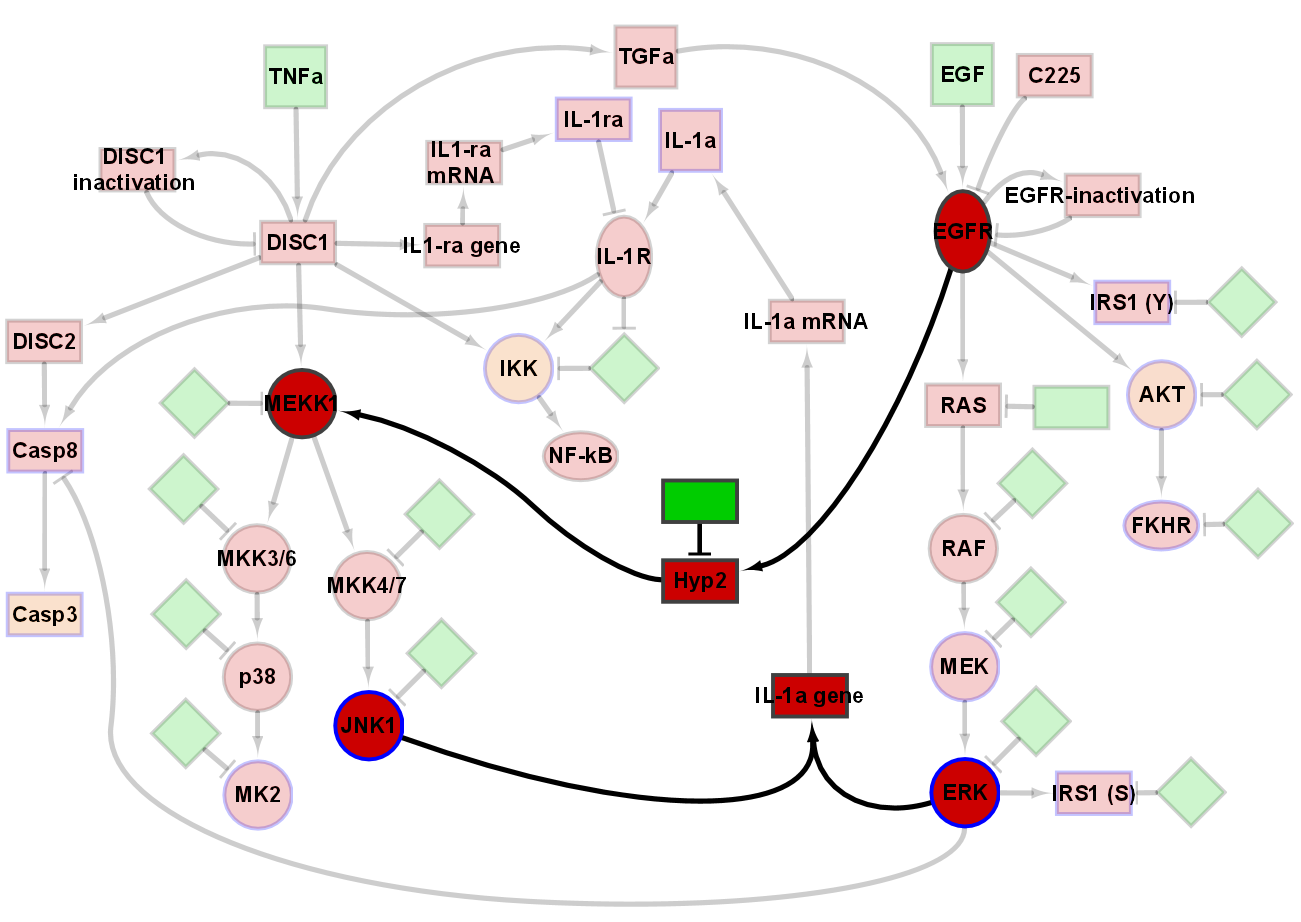
\includegraphics[scale=\largeModelScale]{images/large_network_hypotheses6}}\\
\subfloat[\label{fig:large-model-complete}]{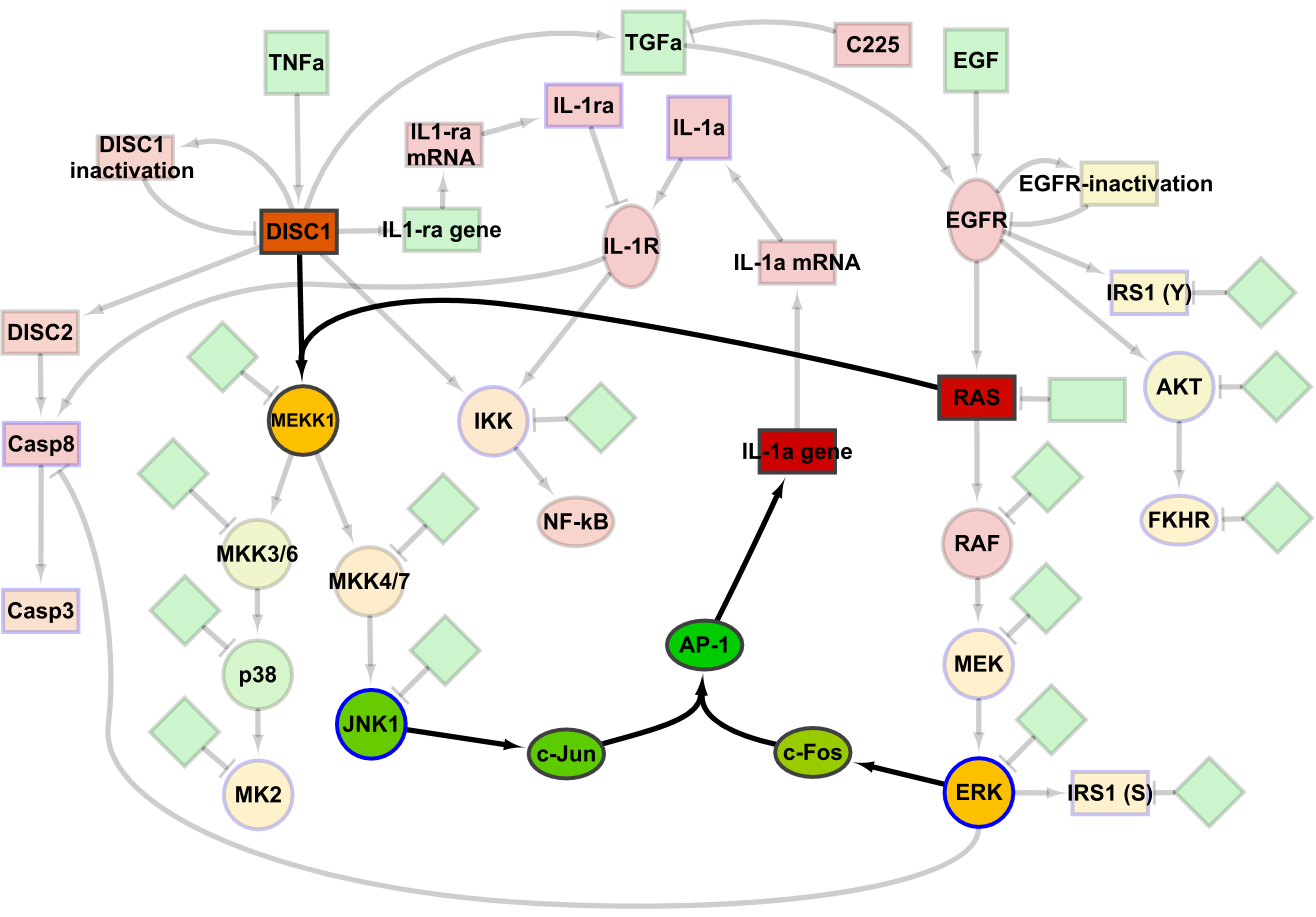
\includegraphics[scale=\largeModelScale]{images/large_network_legendg}}
\\
 \subfloat{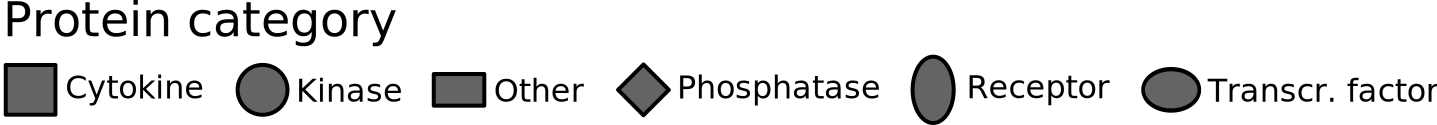
\includegraphics[scale=\legendScalaColori]{images/legenda_forme}}\\ \subfloat{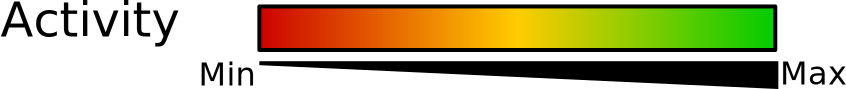
\includegraphics[scale=\legendScalaForme]{images/legenda_colori}}
\caption{ Signaling network downstream of TNF$\alpha$ and EGF in human colon carcinoma cells.
{\bf \protect\subref{fig:large-model-hypotheses}} The merged model for the TNF$\alpha$-EGF pathway in which the two hypotheses are highlighted. Node colors represent initial activity levels.
{\bf \protect\subref{fig:large-model-complete}} The TNF$\alpha$-EGF model with the modified hypotheses. Node colors represent the activity levels $15$ minutes
after stimulation of 100 ng/ml TNF$\alpha$ + 100 ng/ml EGF.}\label{fig:large-model-all}
\end{figure}


Experimentally,
treatment with only TGF$\alpha$ does not lead to secretion of IL-1$\alpha$, for which
 TNF$\alpha$ is also required~\citep{pathway-autocrine}.
However, in the first version of the model TGF$\alpha$ treatment was sufficient for
 IL-1$\alpha$ expression (Fig.~\ref{fig:large-model-graph1}). Given the time delay until secretion of IL-1$\alpha$, it can be
 expected that \emph{de novo} synthesis of IL-1$\alpha$ is required and that both
 TNF$\alpha$ and TGF$\alpha$ are needed to activate transcription of the IL-1$\alpha$ gene.
 JNK1 and ERK signal downstream of TNF$\alpha$ and TGF$\alpha$, respectively, and are known
to affect the activity of many transcription factors. We altered the model to make
 activation of IL-1$\alpha$ expression dependent on both JNK1 activity and ERK activity
(Fig.~\ref{fig:large-model-hypotheses}, arrows linking {\sf JNK1} and {\sf ERK} to {\sf IL-1a gene}).
 After this modification to the model, IL-1$\alpha$ was no longer secreted
upon stimulation with TGF$\alpha$ alone, which greatly improved the fit between the measured IL-1$\alpha$ levels and the model (see
 Fig.~\ref{fig:large-model-graph2}). This hypothesis of IL-1$\alpha$ as a target of combined JNK1 activity and
 ERK activity is supported in literature. Transcription factors c-Jun and c-Fos together
 form a heterodimer known as AP-1 and are activated by JNK1 and ERK,
respectively~\citep{jnk-signaling,cfos-cjun}. AP-1 has been reported to bind to the
 promoter of IL-1$\alpha$, supporting its role in the regulation of IL-1$\alpha$
 expression~\citep{ap1-il1a}. Based on these findings in literature we included c-Jun and
c-Fos in our model as transcriptional activators of IL-1$\alpha$ (Fig.\ref{fig:large-model-complete}).


\begin{figure}[!tpb]
\begin{center}
 \subfloat[\label{fig:large-model-graph1}]{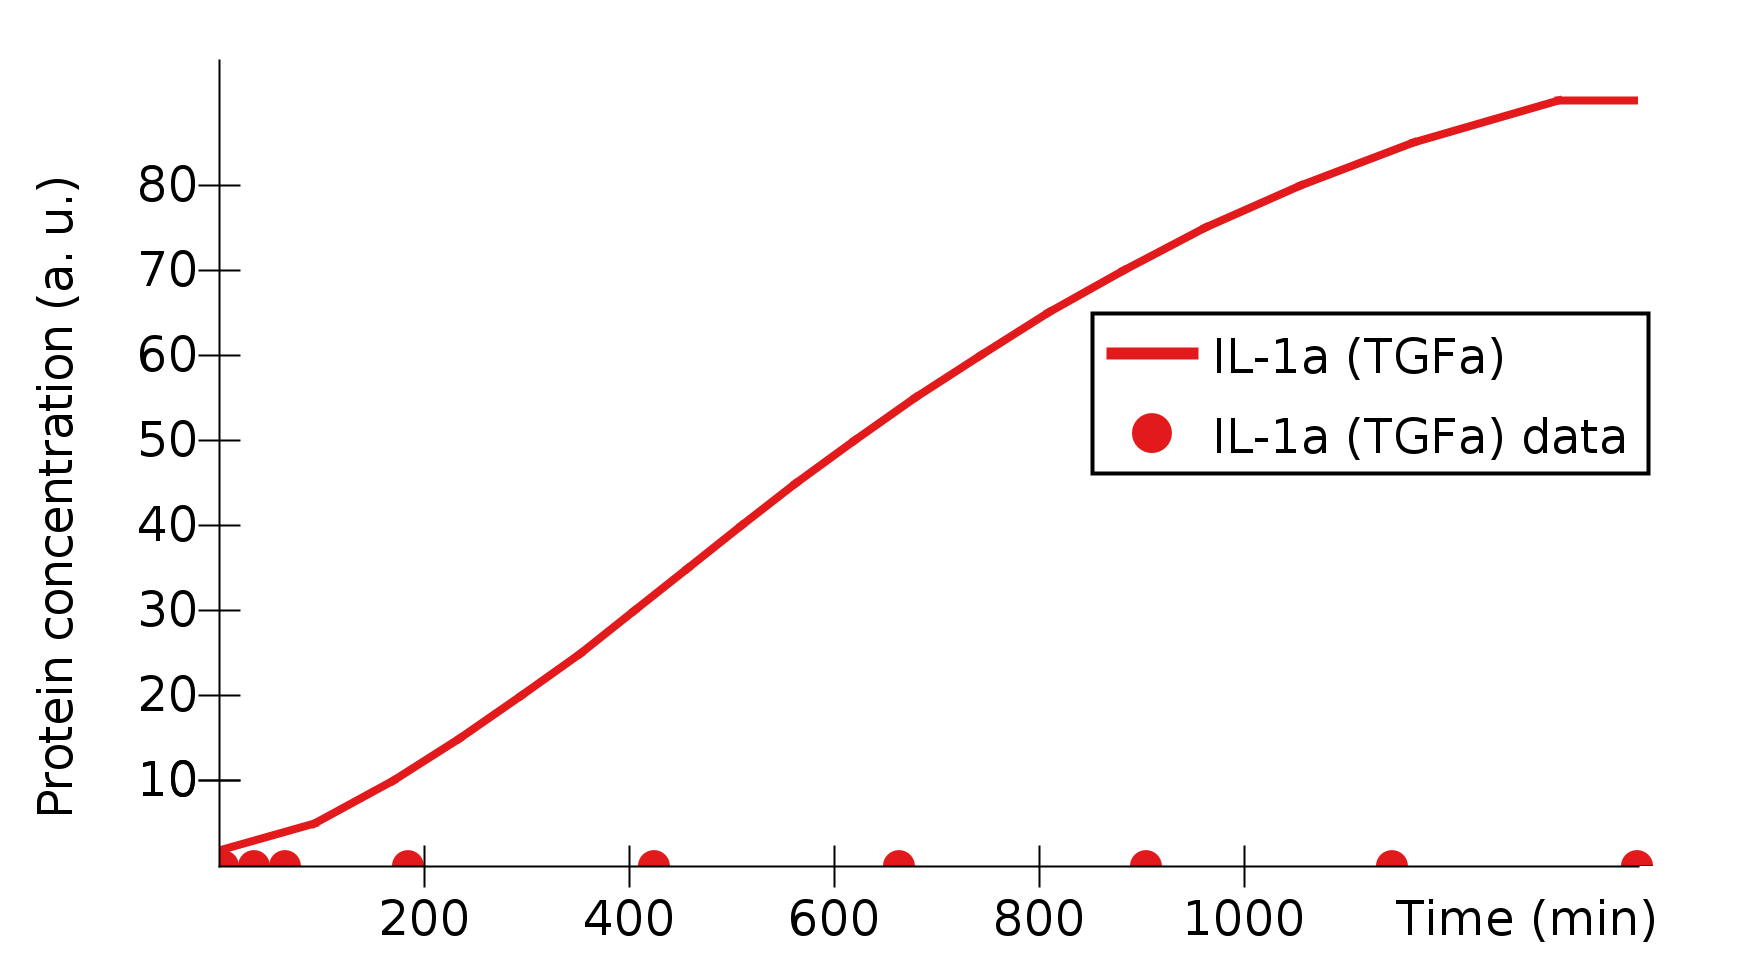
\includegraphics[scale=\scalaGrafici]{images/TGF100_TNF0_ho_hyp_IL-1a3}}
 \subfloat[\label{fig:large-model-graph2}]{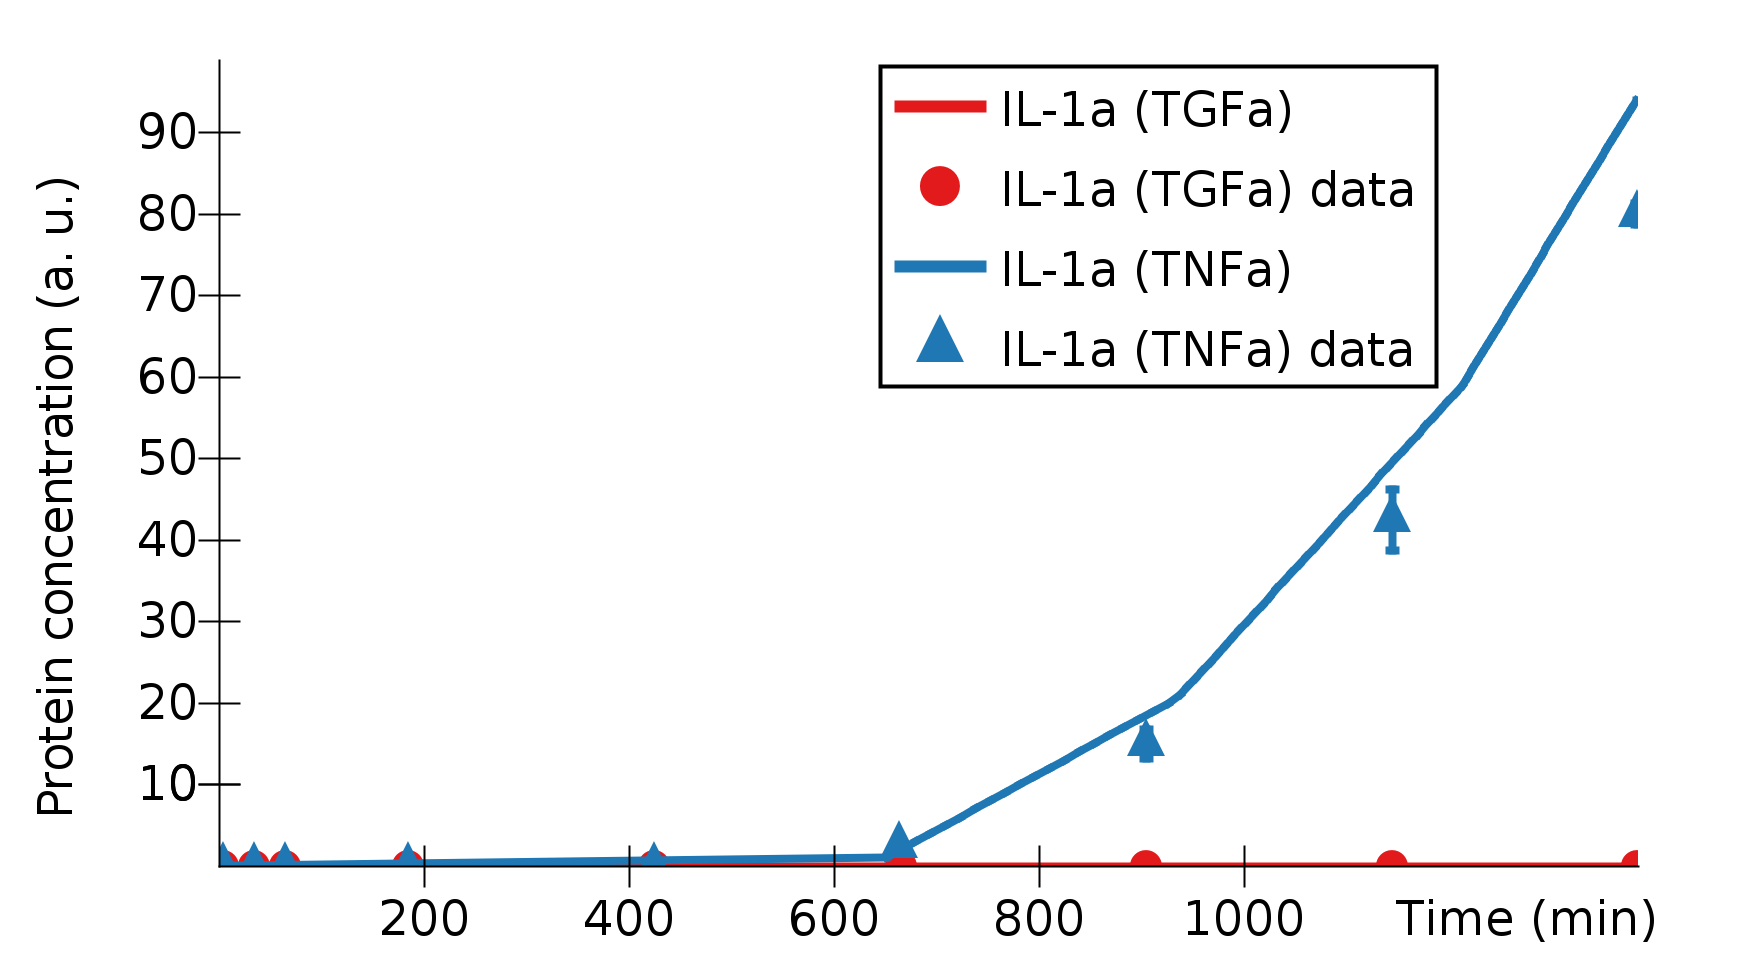
\includegraphics[scale=\scalaGrafici]{images/TGF100_vs_TNF100_hyp1_IL-1a4}}\\
 \subfloat[\label{fig:large-model-graph3}]{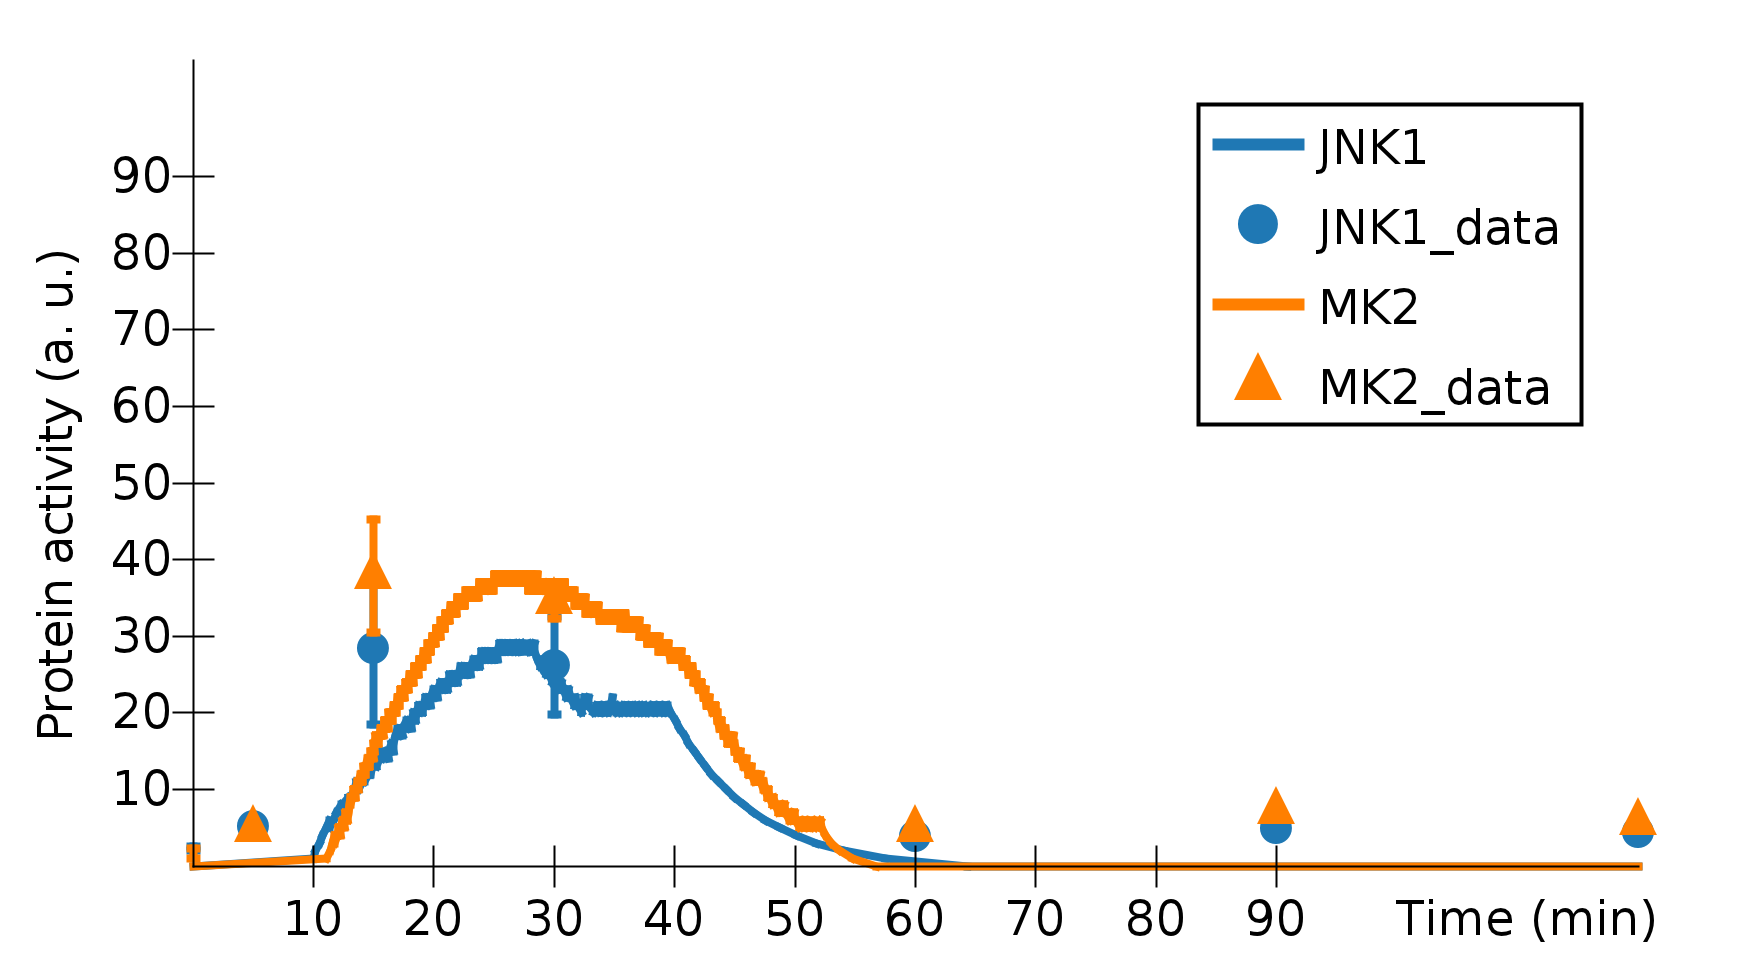
\includegraphics[scale=\scalaGrafici]{images/TNF5_hyp2_JNk1_MK2_3}}
 \subfloat[\label{fig:large-model-graph4}]{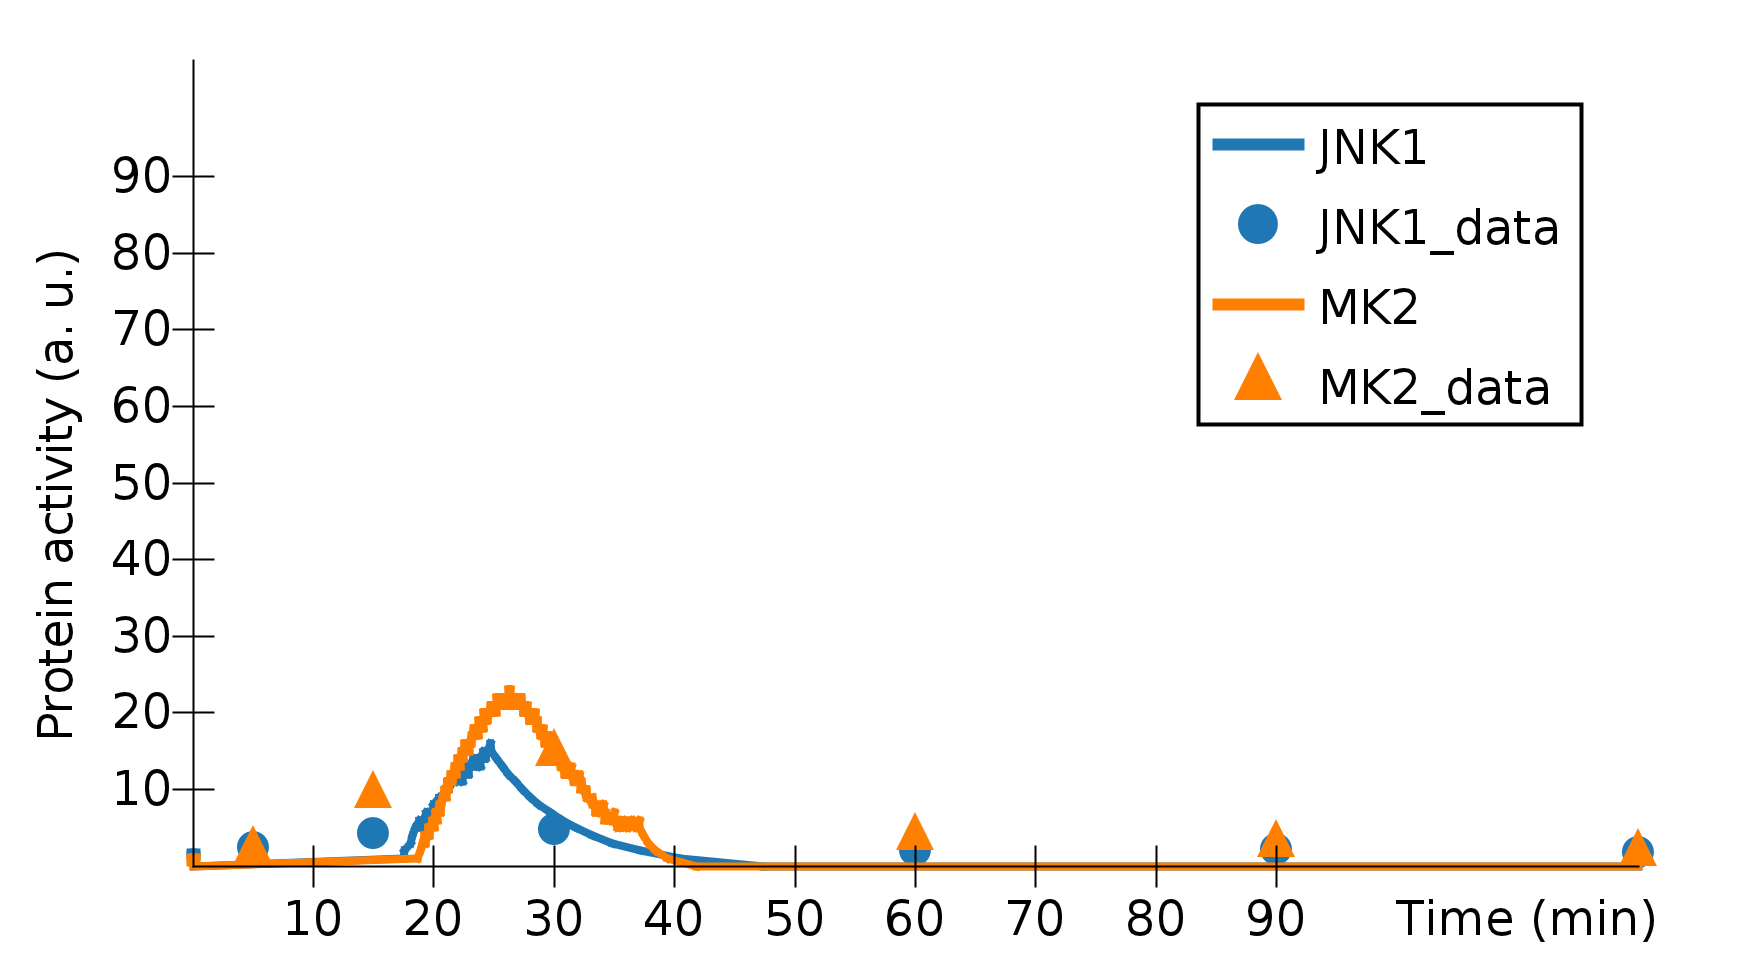
\includegraphics[scale=\scalaGrafici]{images/TNF5_C225_hyp2_JNk1_MK2_3}}
\end{center}
\caption{\scriptsize
Comparison of simulation data obtained from the ANIMO model with experimental data.
{\bf \protect\subref{fig:large-model-graph1}}~Modeled production of IL-1$\alpha$ after stimulation with 100 ng/ml TGF$\alpha$ (24 hours).
{\bf \protect\subref{fig:large-model-graph2}}~After the addition of the first hypothesis (activation of IL-1$\alpha$ production depending both
on JNK1 and ERK): production of IL-1$\alpha$ after stimulation with 100 ng/ml TNF$\alpha$ (series {\sf IL-1a~(TNFa)})
compared with stimulation with 100 ng/ml TGF$\alpha$ (series {\sf IL-1a~(TGFa)}) (24 hours).\\
After the addition of the second hypothesis (activation of MEKK1 downstream of EGFR): {\bf \protect\subref{fig:large-model-graph3}}~stimulation with 5 ng/ml TNF$\alpha$ (2 hours),
{\bf \protect\subref{fig:large-model-graph4}}~stimulation with 5 ng/ml TNF$\alpha$ + 10 $\mu$g/ml C225 (2 hours).}\label{fig:large-model-graph}
\end{figure}


As a second example we considered the behavior of JNK1 and MK2. In the model, both
 proteins were located downstream of TNF$\alpha$ but not TGF$\alpha$ or EGF. Hence, the
 model did not show an effect of C225, a pharmacological inhibitor of ligand-EGFR
 binding, on activation of JNK1 or MK2 after stimulation with TNF$\alpha$. However, experimental
data show that C225 strongly reduces activation of JNK1 and MK2 upon stimulation with TNF$\alpha$~\citep{pathway-autocrine}.
This fact is indicative of a role for EGFR in activation of JNK1 and MK2. Since both JNK1 and MK2
 are located downstream of MAPK/ERK kinase kinase 1 (MEKK1), we hypothesized that activation
 of MEKK1 is dependent on
 both TNF$\alpha$-signaling and TGF$\alpha$-signaling. In the model we added a new
 hypothetical node {\sf Hyp~2} (hypothesis~2) to link EGFR to MEKK1 (Fig~\ref{fig:large-model-hypotheses}).
This addition led to an improved fit of the model to the data upon treatment with TNF$\alpha$ + C225, while preserving the fit
for the other conditions~(Figs.~\ref{fig:large-model-graph3}, \ref{fig:large-model-graph4}). Activation of both MK2 and JNK1
was then strongly suppressed by C225 (Fig.~\ref{fig:large-model-graph4}).
 Stimulation with EGF alone did not lead to activation of JNK1 and MK2.
These data support the validity of the modification to the model.
 Further support for a link between EGFR and MEKK1 was found in literature. Specifically,
Ras GTPase-activating protein (Ras) has been reported as a direct activator of
 MEKK1~\citep{ras-mekk1}. EGFR is a well-known and potent activator of Ras,
 which is why it was already in our network~\citep{kegg}.
Other studies also report activation of JNK1 and phosphorylation of c-Jun downstream of Ras, which is consistent with
 an interaction between Ras and MEKK1~\citep{cfos-cjun,ras-jnk1}.
Based on these findings, we adapted
 our model by removing the {\sf Hyp~2} node and creating a direct interaction between Ras
 and MEKK1 (Fig.~\ref{fig:large-model-complete}). Together, our model suggests that EGFR activity is required but not sufficient for
 activation of JNK1 and MK2 in HT-29 cells.


There are other nodes for which the experimental data deviates from the model in one or more of the experimental conditions.
A comparison between model and experimental data can be found in Figures~\ref{fig:differences1}, \ref{fig:differences2} and~\ref{fig:differences3}.
A complete deciphering of the signaling events
in this biological system is outside the scope of this paper. Instead, we illustrated how interactive modeling of the dynamic behavior
of a signal transduction network can be used to extend previous pathway topologies and can lead to the generation of novel hypotheses.
